\documentclass[a4j,dvipdfmx]{jsarticle}

\usepackage[dvipdfmx]{graphicx}
\usepackage{amsmath}
\usepackage{ascmac, fancybox}
\usepackage{./exp5}

\usepackage{tikz}
\usepackage{subcaption}
\usepackage{float}
\usepackage{amsthm}

% 定理見出し：名前と文献番号を丸括弧なしで併記するスタイル
\newtheoremstyle{plainnote}%
  {}{}%
  {}%                本文フォント（通常）
  {}%
  {\bfseries}%       見出しフォント（太字）
  {}%               見出し後の句読点（なし）
  {.5em}%            見出しと本文の空き
  {\thmname{#1}\thmnumber{ #2}\thmnote{\normalfont\ #3}}% 括弧なしで note を併記

\theoremstyle{plainnote}
\newtheorem{theorem}{定理}[section]
\newtheorem{proposition}[theorem]{命題}
\newtheorem{corollary}[theorem]{系}


%%
%  ここから本文
%%
\begin{document}
\section{序論}

\subsection{背景}
金（Gold）は古くから価値保存手段として扱われ，現代でもインフレや地政学的リスクに応じて価格が変動する重要な資産である。ドル建て金価格は国際的な指標として投資判断やリスク管理に用いられており，その値動きを定量的に捉えるモデル化は実務・学術の両面で関心が高い。

金融時系列を確率過程としてモデル化する枠組みは数多く提案されているが，相関付きランダムウォークモデルは，「直前の値動きの方向」に依存して次の方向を確率的に決めることにより，系列の持続性や反転傾向を少数のパラメータで表現できる点で特徴的である。また，Konno~\cite{ref3} により，量子ウォークに基づく時系列解析のモデルが提案されている。本研究で用いる手法は，このモデルを相関付きランダムウォークに応用して構成した時系列モデルである。

しかし，このような時系列モデルを金価格の値動きに実際に当てはめた先行研究は，筆者の知る限り存在しない。そこで本研究では，相関付きランダムウォークに基づく時系列モデルを金価格の時系列データに適用し，金価格変動の分析における有用性を検討する。

\subsection{目的}
本研究の目的は，相関付きランダムウォークに基づく時系列モデルが金価格の値動きを記述する上でどの程度妥当であるか，またどのような限界を持つのかを実証的に明らかにすることである。具体的には，まず，XAUUSD（ドル建て金価格）の実価格データを平均練行足を用いて離散化し，一定の値幅ごとの上昇・下降からなる値動きの系列を得る。次に，Konno~\cite{ref3} の量子ウォークによる時系列モデルを相関付きランダムウォークに応用した時系列モデルを，この系列に当てはめて次時刻の値を予測する。さらに，予測値と実測値を同一の図上で比較して予測が値動きに追従できているかを視覚的に確認し，補助的な指標として平均絶対誤差（MAE）を併せて評価する。最後に，これらの結果を踏まえ，本モデルが金価格の値動きを記述する上での妥当性と限界について考察する。


\section{確率論}

本章では，以降の議論で用いる確率論の基本概念を整理する。
具体的には，確率空間，確率変数，および独立同分布の定義を述べる。

%---------------------------------------------------------
\subsection{確率空間}
%---------------------------------------------------------

確率現象を数学的に扱うため，以下の三つ組
\[
  (\Omega,\mathcal{F},P)
\]
を考える。これを\textbf{確率空間}という。各構成要素の意味は次の通りである。

\begin{itemize}
  \item $\Omega$：起こり得るすべての結果からなる集合。\textbf{標本空間}とよばれ，その要素 $\omega \in \Omega$ を\textbf{標本点}という。
  \item $\mathcal{F}$：$\Omega$ の部分集合からなる族で，確率を割り当てる対象となる集合の集まり。$\mathcal{F}$ の要素を\textbf{事象}とよぶ。
  \item $P$：$\mathcal{F}$ から $[0,1]$ への関数で，各事象に確率を対応させる。これを\textbf{確率測度}とよぶ。
\end{itemize}

事象の族 $\mathcal{F}$ は，$\Omega$ 上の\textbf{$\sigma$-集合体}でなければならない。
すなわち，以下の三条件を満たす。
\begin{enumerate}
  \item $\Omega\in\mathcal{F}$ である。
  \item $A\in\mathcal{F}$ ならば $\bar{A}\in\mathcal{F}$ である
        （ここで $\bar{A}$ は $A$ の補集合）。
  \item $\mathcal{F}$ の元からなる列 $(A_n,\,n\geq 1)$ に対して，その和集合が
        $\displaystyle\bigcup_{n=1}^{\infty}A_n\in\mathcal{F}$ を満たす。
\end{enumerate}

確率測度 $P$ は，以下の三条件を満たす関数として定義される。
\begin{enumerate}
  \item 任意の $A\in\mathcal{F}$ に対して $P(A)\geq 0$ である。
  \item $P(\Omega)=1$ である。
  \item $A_1,A_2,\ldots \in \mathcal{F}$ が互いに素ならば
        $\displaystyle P\!\left(\bigcup_{i=1}^{\infty} A_i\right)
        =\sum_{i=1}^{\infty}P(A_i)$ が成り立つ。
\end{enumerate}

例えば，1 枚のコインを 1 回投げる試行を考えると，
標本空間は $\Omega=\{\text{表},\text{裏}\}$，
事象の集合は $\mathcal{F}=\{\emptyset,\{\text{表}\},\{\text{裏}\},\Omega\}$，
公平なコインの場合の確率測度は $P(\{\text{表}\})=P(\{\text{裏}\})=1/2$ となる。

%---------------------------------------------------------
\subsection{確率変数}
%---------------------------------------------------------

確率空間 $(\Omega,\mathcal{F},P)$ 上で定義された関数
\[
  X:\Omega \longrightarrow \mathbf{R}
\]
であって，任意の実数 $a$ に対し
\[
  \{\omega \in \Omega \mid X(\omega)\leq a\} \in \mathcal{F}
\]
を満たすものを\textbf{確率変数}という。
ここで，$\mathbf{R}$ は実数全体の集合を表す。
これは，標本空間の各点 $\omega$ に対して実数値 $X(\omega)$ を対応させる関数であり，
かつ $X$ の値に関する事象の確率が定まるものである。

確率変数 $X$ の取り得る値が高々可算個であるとき，$X$ を\textbf{離散確率変数}とよぶ。
本研究で扱う確率変数はすべて離散確率変数である。

確率変数 $X$ に対し，事象 $\{\omega\in\Omega\mid X(\omega)=x\}$ の確率を簡略に
\[
  P(X=x)
\]
と書く。対応 $x \mapsto P(X=x)$ を $X$ の\textbf{確率分布}という。

%---------------------------------------------------------
\subsection{独立性と同分布}\label{subsec:iid}
%---------------------------------------------------------

確率変数列 $X_1,X_2,\ldots,X_n$ が\textbf{独立}であるとは，
任意の実数 $x_1,x_2,\ldots,x_n$ に対して
\begin{equation}
  P(X_1=x_1,\,X_2=x_2,\,\ldots,\,X_n=x_n)
  =\prod_{k=1}^{n} P(X_k=x_k)
  \label{eq:independence}
\end{equation}
が成立するときをいう。
直感的には，ある $X_k$ の実現値が他の $X_j$ ($j\neq k$) の確率分布に影響を与えないことを意味する。

また，確率変数 $X_1,X_2,\ldots,X_n$ が\textbf{同分布}であるとは，
任意の実数 $x$ に対して
\begin{equation}
  P(X_1=x)=P(X_2=x)=\cdots=P(X_n=x)
  \label{eq:identical}
\end{equation}
が成立するときをいう。すなわち，すべての $X_k$ が同一の確率分布に従うことを意味する。

確率変数列 $X_1,X_2,\ldots,X_n$ が独立であり，かつ同分布であるとき，
これを\textbf{独立同分布}（independent and identically distributed，i.i.d.）であるという。

例えば，公平なコインを繰り返し投げ，$k$ 回目に表が出れば $T_k=+1$，
裏が出れば $T_k=-1$ と定めたとき，
$\{T_n\}_{n\geq 1}$ は独立同分布な確率変数列となる。





\newpage
\section{ランダムウォークについて}
\subsection{ランダムウォークの定義}
%---------------------------------------------------------

確率変数列 $\{T_n\}_{n \geq 1}$ を考え，各 $T_n$ は独立同分布で
\begin{equation}
  P(T_n = -1) = p, \quad P(T_n = 1) = q, \qquad (p + q = 1) \label{eq:rv}
\end{equation}
を満たすとする。
これは，\ref{subsec:iid}節の例で導入した公平なコイン投げの列を一般の確率 $p,\,q$ に拡張したものであり，$p = q = 1/2$ の場合が公平なコイン投げに対応する。
このとき，時刻 $n$ におけるランダムウォークの位置 $S_n$ を
\begin{equation}
  S_n = \sum_{k=1}^{n} T_k \label{eq:Sn}
\end{equation}
と定義する。ただし初期位置は $S_0 = 0$ とする。

この定義から，$S_n$ は $n$ 回の独立な試行の結果として定まる確率変数である。
実際，左方向（$T_k = -1$）への移動回数を $\ell$，右方向（$T_k = +1$）への移動回数を $m$ とすると，
$\ell + m = n$ が成り立ち，このとき位置は
\begin{equation}
  x = m - \ell \label{eq:pos}
\end{equation}
で表される。

%---------------------------------------------------------
\subsection{ランダムウォークの確率分布}
%---------------------------------------------------------

次に，時刻 $n$ における位置 $S_n$ の確率分布 $P(S_n = x)$ を考える。
$S_n = x$ が成立するためには，左方向への移動回数 $\ell$ と右方向への移動回数 $m$ が
\begin{equation}
  m - \ell = x, \qquad \ell + m = n \label{eq:lm}
\end{equation}
を満たす必要がある。

$T_n$ が独立であることから，左方向へ $\ell$ 回，右方向へ $m$ 回移動する確率は
$\binom{n}{\ell} p^\ell q^m$ で与えられる。
ここで $\binom{n}{k}$ は，$n$ 個のものから順序を考えずに $k$ 個を選ぶ場合の数を表す
\textbf{二項係数}であり，
\begin{equation}
  \binom{n}{k} = {}_n C_k = \frac{n!}{k!\,(n-k)!}
  \qquad (0\leq k\leq n)
  \label{eq:binom}
\end{equation}
で定義される。すなわち $\binom{n}{k}$ は，高校数学などで用いられる組合せの記号 ${}_n C_k$ と同じものである。
したがって，事象「$S_n = x$」の確率は
\begin{equation}
  P(S_n = x) = \binom{n}{\ell} p^\ell q^m
  = \frac{n!}{\ell!\,(n-\ell)!}\,p^\ell q^m
  \label{eq:dist}
\end{equation}
で与えられる。ただし $\ell = (n-x)/2$，$m = (n+x)/2$ とする
（$(n+x)/2$ が非負整数でないとき $P(S_n=x)=0$ とする）。

例えば，時刻 $n = 1$ のときは
\begin{equation}
  P(S_1 = -1) = p, \qquad P(S_1 = 1) = q \label{eq:n1}
\end{equation}
となる。同様にして時刻 $n = 2$ のときは
\begin{equation}
  P(S_2 = -2) = p^2, \qquad P(S_2 = 0) = 2pq, \qquad P(S_2 = 2) = q^2
  \label{eq:n2}
\end{equation}
となる。
このときの時刻 $n=1,2$ における遷移と確率を
図\,\ref{fig:rw_transition} に示す。


\begin{figure}[H]
  \centering
  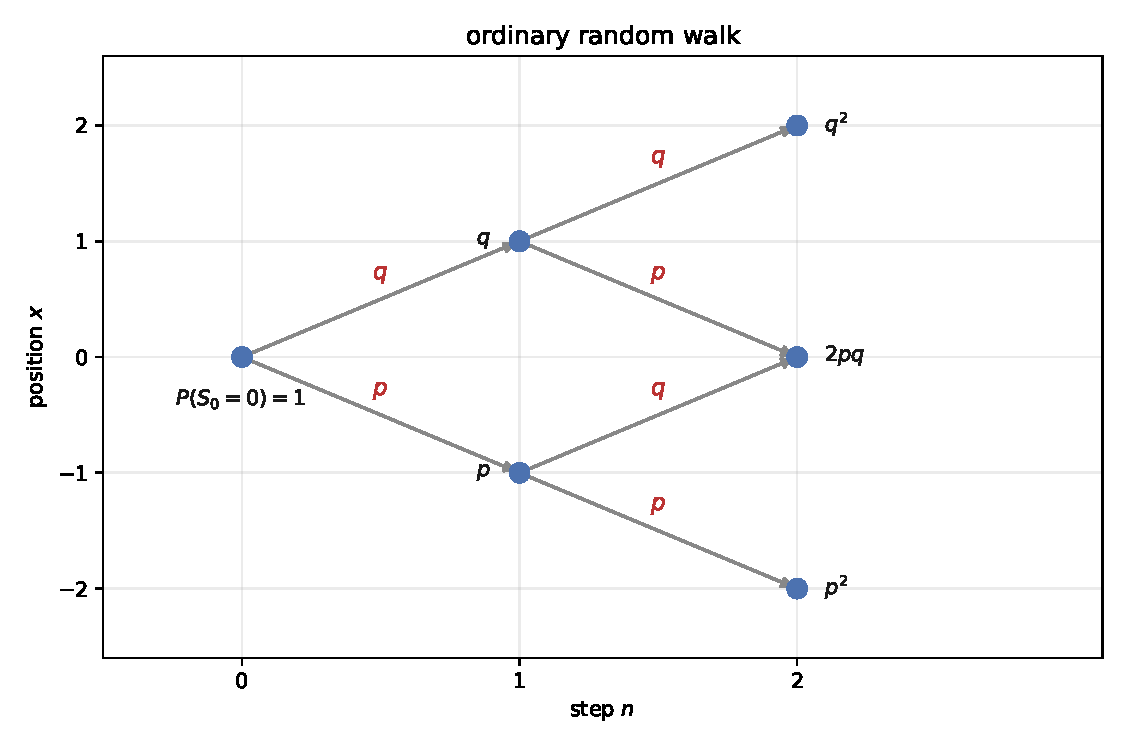
\includegraphics[width=\textwidth]{rw_transition}
  \caption{ランダムウォークの遷移と確率}
  \label{fig:rw_transition}
\end{figure}



さらに，$n = 3$ のときは
\begin{align}
  P(S_3 = -3) = \binom{3}{3} p^3 q^0 = p^3, &\qquad
  P(S_3 = -1) = \binom{3}{2} p^2 q^1 = 3p^2 q, \label{eq:n3a}\\
  P(S_3 = 1)  = \binom{3}{1} p^1 q^2 = 3pq^2, &\qquad
  P(S_3 = 3)  = \binom{3}{0} p^0 q^3 = q^3   \label{eq:n3b}
\end{align}
となる。

また，対称なランダムウォークの場合は
\[
  p=q=\frac{1}{2}
\]
である。このときの時刻 $n=1,2,3,4$ における確率分布を
図\,\ref{fig:rw_barchart} に示す。
\begin{figure}[htbp]
  \centering
  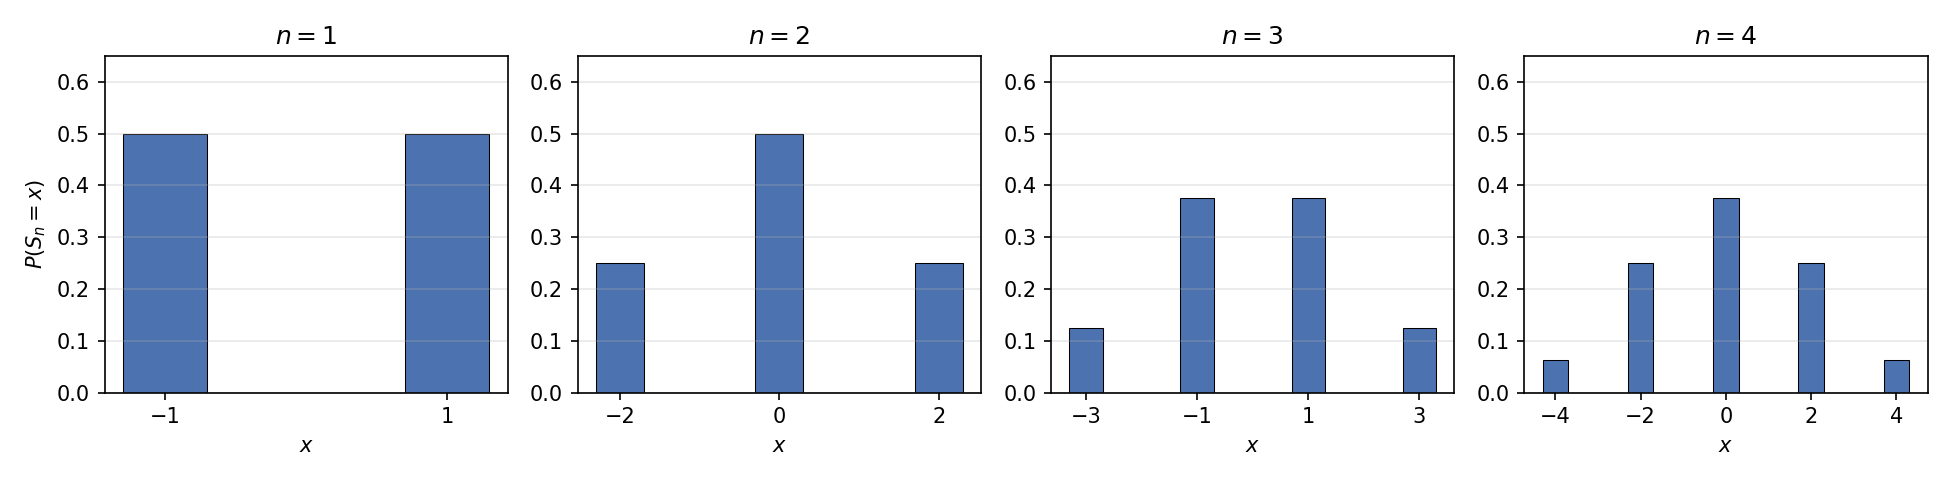
\includegraphics[width=\textwidth]{rw_barchart.png}
  \caption{対称ランダムウォーク（$p=q=\frac{1}{2}$）における時刻 $n=1,2,3,4$ の確率分布}
  \label{fig:rw_barchart}
\end{figure}

%---------------------------------------------------------
\subsection{ランダムウォークの極限分布}
%---------------------------------------------------------

本節では，1次元ランダムウォークに関する代表的な極限定理を紹介する。
まず，以下の\textbf{大数の法則}が成り立つ。

\begin{theorem}[大数の法則~{\cite{ref1}}]
\label{thm:lln}
\begin{equation}
  P\!\left(\lim_{n \to \infty} \frac{S_n}{n} = q - p\right) = 1
  \label{eq:lln}
\end{equation}
が成立する。
\end{theorem}

さらに，以下の\textbf{中心極限定理}が成り立つ。

\begin{theorem}[中心極限定理~{\cite{ref1}}]
\label{thm:clt}
$pq \neq 0$ とする。このとき $-\infty < a < b < \infty$ に対し，
\begin{equation}
  \lim_{n \to \infty} P\!\left(a \leq \frac{S_n - (q-p)n}{\sqrt{4pqn}} \leq b\right)
  = \int_a^b \frac{1}{\sqrt{2\pi}}\,e^{-x^2/2}\,dx
  \label{eq:clt}
\end{equation}
が成立する。
\end{theorem}

この結果は，ランダムウォークの極限の確率変数が平均 $0$，分散 $1$ の正規分布に従うことを意味する。
ここで，確率変数 $S$ が平均 $m$，分散 $v$ の正規分布に従うとは，
\begin{equation}
  P(a \leq S \leq b) = \int_a^b \frac{1}{\sqrt{2\pi v}}\,e^{-(x-m)^2/(2v)}\,dx
  \qquad (a < b)
  \label{eq:normal_def}
\end{equation}
を満たすときをいう。ただし $m$ は実数，$v$ は正の実数である。

一般に，確率変数列 $\{X_1, X_2, X_3, \ldots\}$ と確率変数 $X$ があり，$X_n$ が $X$ に\textbf{弱収束する}とは，任意の $a < b$ に対し
\begin{equation}
  \lim_{n \to \infty} P(a \leq X_n \leq b) = P(a \leq X \leq b)
  \label{eq:weak_conv}
\end{equation}
が成立するときをいう。$X_n$ が $X$ に弱収束することを $X_n \Rightarrow X$ と表す。また，このような極限定理を\textbf{弱収束極限定理}という。
定理\,\ref{thm:clt}より，対称な $p = q = 1/2$ の場合は以下の系が導かれる。

\begin{corollary}
\label{cor:clt_sym}
$-\infty < a < b < \infty$ に対し，
\begin{equation}
  \lim_{n \to \infty} P\!\left(a \leq \frac{S_n}{\sqrt{n}} \leq b\right)
  = \int_a^b \frac{1}{\sqrt{2\pi}}\,e^{-x^2/2}\,dx
  \label{eq:clt_sym}
\end{equation}
が成立する。
\end{corollary}

ランダムウォーク $S_n$ の場合，スケーリングは $S_n/\sqrt{n}$ のように $\sqrt{n}$ で割る形となる。極限の標準正規分布を図示すると図\,\ref{fig:normal} のようになる。


\begin{figure}[H]
  \centering
  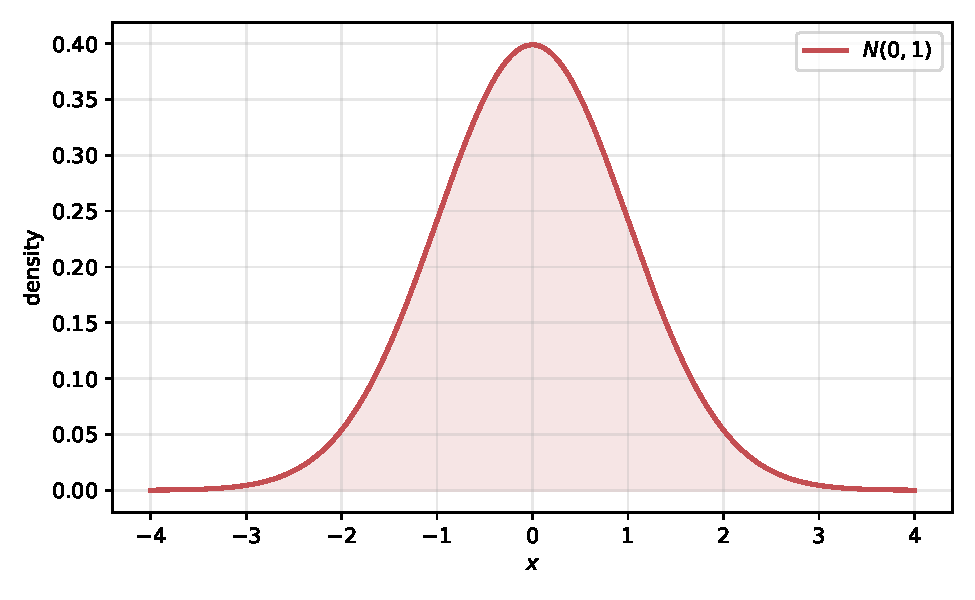
\includegraphics[width=0.75\textwidth]{normal_limit_distribution}
  \caption{ランダムウォークの極限測度（標準正規分布）}
  \label{fig:normal}
\end{figure}
\newpage

\section{相関付きランダムウォークについて}
%%%%%%%%%%%%%%%%%%%%%%%%%%%%%%%%%%%%%%%%%%%%%%%%%%%%%%%%%%%

\subsection{相関付きランダムウォークの定義}

通常のランダムウォークでは各ステップが独立であるが，
\textbf{相関付きランダムウォーク}では
直前の移動方向が次のステップの確率に影響する。


パラメータ $a, b, c, d \in (0,1)$，$a + c = b + d = 1$ を固定する。
各ステップの条件付き確率を
\begin{align*}
  P(\text{左} \mid \text{直前：左}) &= a, \quad &
  P(\text{右} \mid \text{直前：左}) &= c = 1-a, \\
  P(\text{左} \mid \text{直前：右}) &= b, \quad &
  P(\text{右} \mid \text{直前：右}) &= d = 1-b
\end{align*}
で定める。このとき定まる確率過程 $(\tilde{S}_n)_{n \geq 0}$ を
\textbf{相関付きランダムウォーク}という。

\subsubsection*{行列による定式化}

内部状態（向き）を，ブラケット記号を用いて
\[
  |L\rangle = \begin{pmatrix}1\\0\end{pmatrix} \text{（左向き）}, \qquad
  |R\rangle = \begin{pmatrix}0\\1\end{pmatrix} \text{（右向き）}
\]
と表す。これを用いて，相関付きランダムウォークを $2 \times 2$ 行列で定式化する。

転置推移確率行列を
\[
  A = \begin{pmatrix} a & b \\ c & d \end{pmatrix}, \qquad
  a + c = b + d = 1, \quad 0 < a,\, d < 1
\]
で定める。これに対して
$A|L\rangle = a|L\rangle + c|R\rangle$，
$A|R\rangle = b|L\rangle + d|R\rangle$
が成り立つ。

次に，時刻 $n$，位置 $x$ における確率ベクトルを
\[
  \Psi_n(x) = \begin{pmatrix} \Psi_n^L(x) \\ \Psi_n^R(x) \end{pmatrix}
\]
で表す。ここで $\Psi_n^L(x)$（resp.\ $\Psi_n^R(x)$）は時刻 $n$ に
左向き（resp.\ 右向き）で位置 $x$ にある確率である。
正規化条件
\[
  \sum_{x \in \mathbf{Z}} \bigl(\Psi_n^L(x) + \Psi_n^R(x)\bigr) = 1
\]
を仮定する。

ここで，2次元ベクトル $v = (v_1, v_2)^\top$ に対する1ノルムを
\begin{equation}
  \|v\|_1 = |v_1| + |v_2|
  \label{eq:l1_norm}
\end{equation}
で定義する。これは，ベクトルの各成分の絶対値の和である。
本研究で扱う確率ベクトル $\Psi_n(x)$ の成分は非負であるため，
$\|\Psi_n(x)\|_1 = \Psi_n^L(x) + \Psi_n^R(x)$ となる。
これを用いて，時刻 $n$ に位置 $x$ にいる確率を
\[
  P(\tilde{S}_n = x) = \Psi_n^L(x) + \Psi_n^R(x) = \|\Psi_n(x)\|_1
\]
で定める。

行列 $A$ を左移動成分 $P$ と右移動成分 $Q$ に分解して
\[
  P = \begin{pmatrix} a & b \\ 0 & 0 \end{pmatrix}, \qquad
  Q = \begin{pmatrix} 0 & 0 \\ c & d \end{pmatrix}, \qquad
  A = P + Q
\]
とする。
$P$ は左向きへの寄与（位置 $x+1$ から $x$ への左向き移動），
$Q$ は右向きへの寄与（位置 $x-1$ から $x$ への右向き移動）を担う。
確率ベクトルの時間発展は
\begin{equation}
  \Psi_{n+1}(x) = P\,\Psi_n(x+1) + Q\,\Psi_n(x-1)
  \label{eq:crw_evolution}
\end{equation}
で与えられる。

初期確率ベクトルを
$\varphi = (\alpha,\,\beta)^\top$，$\alpha + \beta = 1$，$\alpha,\beta \geq 0$
とし，初期状態は原点 $\Psi_0(0) = \varphi$ とする。
$\alpha = 0$（resp.\ $\beta = 0$）は右向き（resp.\ 左向き）から出発することに対応する。

%---------------------------------------------------------
\subsection{相関付きランダムウォークの確率分布}
%---------------------------------------------------------

\subsubsection*{パス和 $\Xi_n(l,m)$}

$n$ ステップで左に $l$ 回，右に $m$ 回（$l + m = n$）移動するとき，
$l$ 個の $P$（左移動行列）と $m$ 個の $Q$（右移動行列）の積の全順序づけの和を
$\Xi_n(l, m)$ で表す。
すなわち，$P$ を $l$ 個，$Q$ を $m$ 個含む長さ $n$ の語全体にわたる行列積の和として
\begin{equation}
  \Xi_n(l, m)
  = \sum_{\substack{(w_1,\ldots,w_n)\in\{P,Q\}^n \\
        \#\{\,i : w_i = P\,\}=l,\;\#\{\,i : w_i = Q\,\}=m}}
    w_1 w_2 \cdots w_n
  \label{eq:path_sum}
\end{equation}
で定義する。ここで $\#\{\cdot\}$ は集合の要素数を表す。
位置と試行回数の関係は $x = m - l$，$l = \dfrac{n-x}{2}$，$m = \dfrac{n+x}{2}$ である。

$n = 2$ の場合は
\begin{align*}
  \Xi_2(2,0) &= P^2, \quad \Xi_2(0,2) = Q^2, \\
  \Xi_2(1,1) &= QP + PQ
\end{align*}
となる。

$n = 3$ の場合は
\begin{align*}
  \Xi_3(3,0) &= P^3, \quad \Xi_3(0,3) = Q^3, \\
  \Xi_3(2,1) &= QP^2 + PQP + P^2Q, \\
  \Xi_3(1,2) &= PQ^2 + QPQ + Q^2P
\end{align*}
となる。

ここで，通常のランダムウォークと相関付きランダムウォークの確率分布の構造的な違いを述べる。
通常のランダムウォークでは，各ステップの確率が直前の状態によらず独立に定まるため，
$P, Q$ がスカラーとなり，左右の移動回数だけで確率が決まる。
このため $\Xi_2(1,1)$ は $2 \times P \times Q$ に対応し，
$n$ ステップで左に $l$ 回，右に $m$ 回移動する確率は，
順序によらず二項係数 $\binom{n}{\ell}$ と $p^\ell q^m$ の積で表される。

一方，相関付きランダムウォークでは $P$ と $Q$ が行列で\textbf{非可換}であるため，
$\Xi_2(1,1) = QP + PQ \neq 2PQ$ が一般に成り立つ。
すなわち，左右の移動回数が同じであっても，移動の順序が異なれば確率が異なる。
このため，相関付きランダムウォークの確率分布は単純な二項係数では表せず，
直前の方向に依存する経路ごとの寄与を行列積として加え合わせる必要がある。
この違いが，相関付きランダムウォーク特有の持続性や反転傾向を生み出す。

時刻 $n$ に位置 $x$ にいる確率は
\begin{equation}
  P(\tilde{S}_n = x) = \|\Xi_n(l,m)\,\varphi\|_1,
  \qquad l = \tfrac{n-x}{2},\; m = \tfrac{n+x}{2}
  \label{eq:crw_Xi}
\end{equation}
で与えられる。$\displaystyle\sum_{x} P(\tilde{S}_n = x) = 1$ を満たす。

\subsubsection*{$n = 1, 2$ の具体計算}

以下では $\varphi = (\alpha, \beta)^\top$（$\alpha + \beta = 1$），
$P = \bigl(\begin{smallmatrix}a&b\\0&0\end{smallmatrix}\bigr)$，
$Q = \bigl(\begin{smallmatrix}0&0\\c&d\end{smallmatrix}\bigr)$ を用いる。

\medskip
\noindent\textbf{$n=1$ のとき}（行列計算の詳細）は
\begin{align*}
  \widetilde{P}(\tilde{S}_1 = -1)
    &= P\varphi
     = \begin{pmatrix} a & b \\ 0 & 0 \end{pmatrix}
       \begin{pmatrix} \alpha \\ \beta \end{pmatrix}
     = \begin{pmatrix} a\alpha + b\beta \\ 0 \end{pmatrix}, \\[4pt]
  \widetilde{P}(\tilde{S}_1 = +1)
    &= Q\varphi
     = \begin{pmatrix} 0 & 0 \\ c & d \end{pmatrix}
       \begin{pmatrix} \alpha \\ \beta \end{pmatrix}
     = \begin{pmatrix} 0 \\ c\alpha + d\beta \end{pmatrix}
\end{align*}
となる。よって
\[
  P(\tilde{S}_1 = -1) = a\alpha + b\beta, \qquad P(\tilde{S}_1 = +1) = c\alpha + d\beta
\]
である。和は $(a+c)\alpha + (b+d)\beta = \alpha + \beta = 1$ となり，確率測度であることが確認できる。

\medskip
\noindent\textbf{$n=2$ のとき}は
\begin{align*}
  P(\tilde{S}_2 = -2) &= a\,(a\alpha + b\beta), \\
  P(\tilde{S}_2 =  0) &= b\,(c\alpha + d\beta) + c\,(a\alpha + b\beta), \\
  P(\tilde{S}_2 = +2) &= d\,(c\alpha + d\beta)
\end{align*}
となる。
このときの時刻 $n=1,2$ における遷移と確率を
図\,\ref{fig:crw_transition} に示す。

\begin{figure}[H]
  \centering
  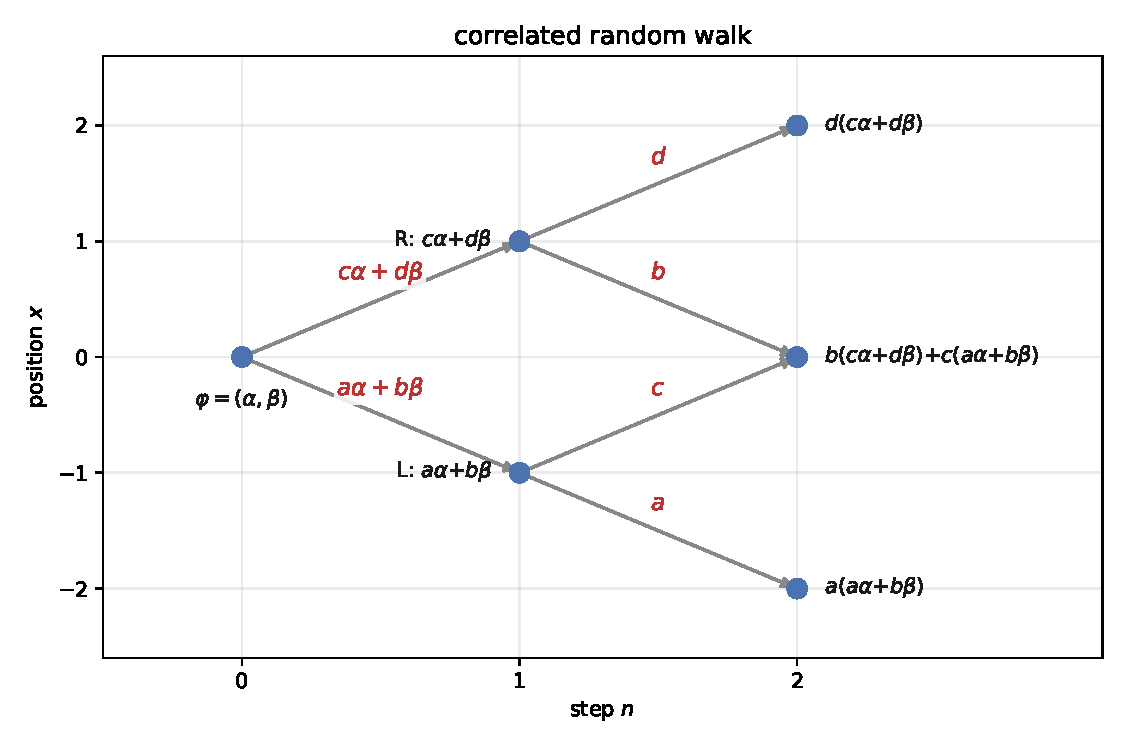
\includegraphics[width=\textwidth]{crw_transition}
  \caption{相関付きランダムウォークの遷移と確率}
  \label{fig:crw_transition}
\end{figure}


上の具体計算をもとに，
\[
  a=d=\frac{2}{3}, \qquad
  b=c=\frac{1}{3}, \qquad
  \alpha=\beta=\frac{1}{2}
\]
の場合の確率分布を図\,\ref{fig:crw_barchart} に示す。
\begin{figure}[htbp]
  \centering
  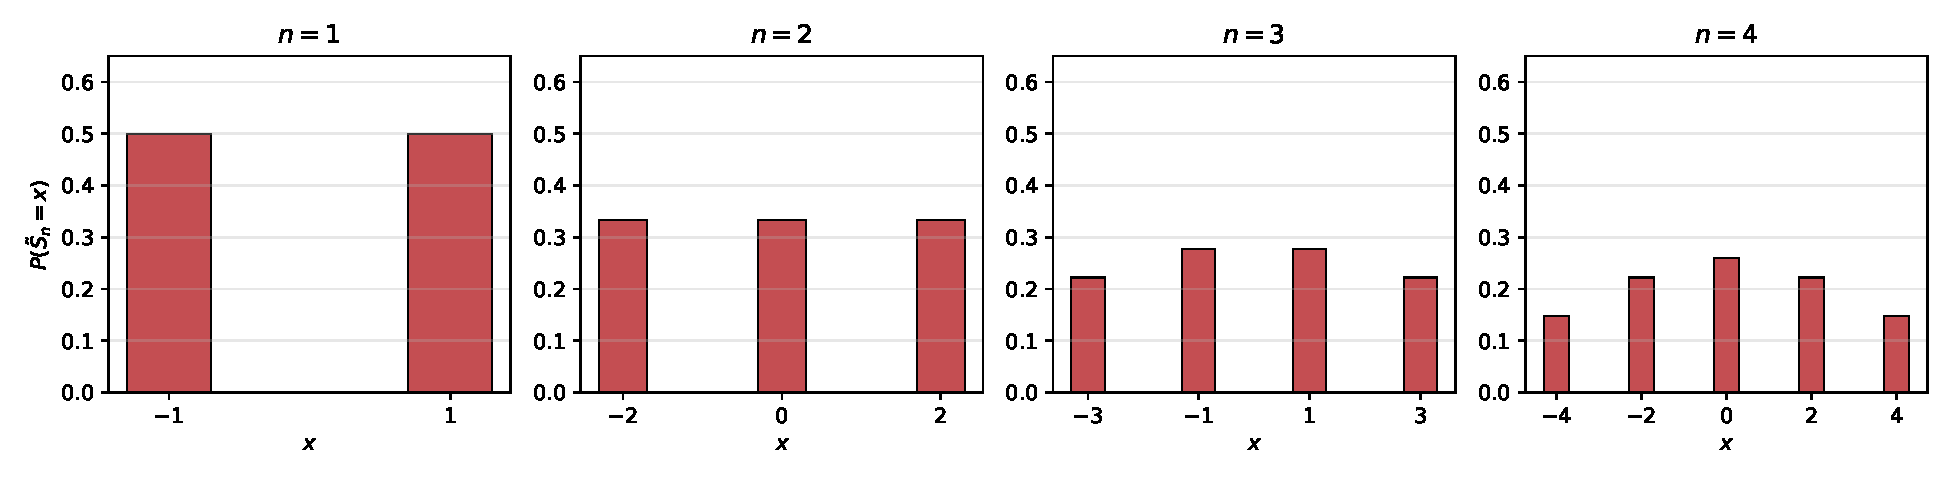
\includegraphics[width=\textwidth]{crw_barchart}
  \caption{相関付きランダムウォーク（$a=d=2/3,\ \alpha=\beta=1/2$）における時刻 $n=1,2,3,4$ の確率分布}
  \label{fig:crw_barchart}
\end{figure}

\subsubsection*{通常のランダムウォークとの確率分布の比較}

ここで，対称な通常のランダムウォーク（$p=q=1/2$）の確率分布（図\,\ref{fig:rw_barchart}）と，
持続性をもつ相関付きランダムウォーク（$a=d=2/3$，$\alpha=\beta=1/2$）の確率分布（図\,\ref{fig:crw_barchart}）を，
同じ時刻 $n=1,2,3,4$ について比較する。
どちらも初期確率ベクトルが対称であるため，分布は原点まわりで左右対称であり，
時刻 $n=1$ ではともに $P(\pm 1)=1/2$ となって完全に一致する。
しかし時刻 $n=2$ では両者の差が現れる。
通常のランダムウォークでは
\[
  P(S_2=0)=2pq=\tfrac{1}{2}, \qquad P(S_2=\pm 2)=\tfrac{1}{4}
\]
であるのに対し，相関付きランダムウォークでは
\[
  P(\tilde{S}_2=0)=\tfrac{1}{3}, \qquad P(\tilde{S}_2=\pm 2)=\tfrac{1}{3}
\]
となり，原点（$x=0$）の確率が小さく，両端（$x=\pm 2$）の確率が大きい。
これは，相関付きランダムウォークでは直前と同じ方向へ進みやすい\textbf{持続性}（$a>1/2$）があるため，
一度動き出した向きにそのまま進んで両端に到達しやすいことを反映している。
この傾向は時刻が進むほど蓄積し，時刻 $n=3,4$ と進むにつれて，
相関付きランダムウォークの分布は通常のランダムウォークの分布よりも
中央が低く，裾が広い（より分散の大きい）形になっていく。
このように，図\,\ref{fig:rw_barchart} と図\,\ref{fig:crw_barchart} を比べると，
左右の移動回数が同じ経路でも順序によって確率が変わるという
相関付きランダムウォークの性質が，分布の広がりの違いとして現れることがわかる。

%---------------------------------------------------------
\subsection{相関付きランダムウォークの極限分布}
%---------------------------------------------------------

本節では，相関付きランダムウォークに関する極限定理を紹介する。
以下では，整数全体の集合を
$\mathbf{Z}=\{\ldots,-2,-1,0,1,2,\ldots\}$，
非負整数全体の集合を
$\mathbf{Z}_{\geq 0}=\{0,1,2,3,\ldots\}$
と表す。
以下のコイン行列で定まる相関付きランダムウォークを考える。
\begin{equation}
  A = \begin{pmatrix} a & b \\ c & d \end{pmatrix}
\end{equation}
ここで，相関付きランダムウォークが\textbf{時間発展対称}であるとは，
$a = d$ かつ $b = c = 1 - a$（$0 < a < 1$）を満たすときをいい，このとき
\begin{equation}
  A = \begin{pmatrix} a & 1-a \\ 1-a & a \end{pmatrix}
  \label{eq:sym_corr_matrix}
\end{equation}
の形になる。この場合，初期確率ベクトルを $\varphi = (1/2,\,1/2)^\top$ にとると，
任意の $n \in \mathbf{Z}_{\geq 0}$ と $x \in \mathbf{Z}$ に対して
$P(\tilde{S}_n = x) = P(\tilde{S}_n = -x)$ が成立し，確率測度は原点まわりで対称となる。

確率測度が原点まわりで対称となる条件について，次がいえる。

\begin{proposition}[{\cite{ref1}}]
\label{prop:symmetry}
\eqref{eq:sym_corr_matrix} で定まる時間発展対称な相関付きランダムウォーク $(\tilde{S}_n)_{n \geq 0}$ について，次が成り立つ。
\begin{enumerate}
  \item 初期確率ベクトルを $\varphi = (1/2,\,1/2)^\top$ にとると，
        任意の $n \in \mathbf{Z}_{\geq 0}$ と $x \in \mathbf{Z}$ に対して
        $P(\tilde{S}_n = x) = P(\tilde{S}_n = -x)$ が成立する。
  \item 特に $a = 1/2$（すなわち $p = a = 1/2$）のときは，初期確率ベクトル $\varphi$ によらず
        （初期条件を問わず），任意の $n \in \mathbf{Z}_{\geq 0}$ と $x \in \mathbf{Z}$ に対して
        $P(\tilde{S}_n = x) = P(\tilde{S}_n = -x)$ が成立する。
\end{enumerate}
\end{proposition}

第5章で構成する相関付きランダムウォークの時系列モデルでは，
初期確率ベクトルはパラメータ $\alpha$ を用いて
$\varphi = (\alpha,\,1-\alpha)^\top$ と表され，
$\alpha$ は特定の値に固定されない。
そこでここでは，初期確率ベクトルによらず対称性が成り立つことを述べた
(2) の場合を確認する。
$a = 1/2$ のとき，コイン行列は
\[
  A = \begin{pmatrix} 1/2 & 1/2 \\ 1/2 & 1/2 \end{pmatrix}, \qquad
  P = \begin{pmatrix} 1/2 & 1/2 \\ 0 & 0 \end{pmatrix}, \qquad
  Q = \begin{pmatrix} 0 & 0 \\ 1/2 & 1/2 \end{pmatrix}
\]
となる。このとき，任意の初期確率ベクトル $\varphi = (\alpha,\,\beta)^\top$（$\alpha + \beta = 1$）に対して
\[
  P\varphi = \begin{pmatrix} (\alpha+\beta)/2 \\ 0 \end{pmatrix} = \begin{pmatrix} 1/2 \\ 0 \end{pmatrix}, \qquad
  Q\varphi = \begin{pmatrix} 0 \\ (\alpha+\beta)/2 \end{pmatrix} = \begin{pmatrix} 0 \\ 1/2 \end{pmatrix}
\]
となり，左右への移動確率はともに $1/2$ で，直前の方向に依存しない。
したがって $a = 1/2$ のときは各ステップが実質的に独立となり，
相関付きランダムウォークは初期の向きによらず対称な通常のランダムウォーク（$p=q=1/2$）に一致するため，
初期確率ベクトル $\varphi$ を問わず確率測度は原点まわりで対称となる。

時間発展対称な相関付きランダムウォークについて，以下の弱収束極限定理が成り立つ。

\begin{theorem}[相関付きランダムウォークの弱収束極限定理~{\cite{ref2}}]
\label{thm:clt_corr}
\eqref{eq:sym_corr_matrix} で定まる時間発展対称な相関付きランダムウォーク $(\tilde{S}_n)_{n \geq 0}$ に対し，$n \to \infty$ とすると
\begin{equation}
  \frac{\tilde{S}_n}{\sqrt{n}} \;\Rightarrow\; W
  \label{eq:clt_corr}
\end{equation}
が成立する。
ここで $W$ の確率測度は $N\!\left(0,\,\dfrac{a}{1-a}\right)$ に従い，
$N(m,\sigma^2)$ は平均 $m$ で分散 $\sigma^2$ の正規分布である。
\end{theorem}

なお，上記の極限測度 $W$ は初期の確率測度 $\varphi$ に依存しないことに注意する。

極限分散 $\sigma^2 = \dfrac{a}{1-a}$ は，対称な通常ランダムウォーク（極限分散 $1$）と比較して，パラメータ $a$ に応じて次のように振る舞う。
\begin{itemize}
  \item $a = 1/2$ のとき，$\sigma^2 = 1$ であり通常ランダムウォークの極限分布と一致する。
  \item $a > 1/2$（持続性）のとき，$\sigma^2 > 1$ となり分布の裾が広い。
  \item $a < 1/2$（反転傾向）のとき，$\sigma^2 < 1$ となり分布の裾が狭い。
\end{itemize}

この定理を数値的に確認するため，時間発展対称な相関付きランダムウォーク
（初期確率ベクトル $\varphi = (1/2,\,1/2)^\top$）について，
式\eqref{eq:crw_evolution} の時間発展を反復して時刻 $n = 100$ における
確率分布 $P(\tilde{S}_n = x)$ を厳密に計算し，
定理\,\ref{thm:clt_corr} と同じ再スケールを施した変数
$u = \tilde{S}_n/\sqrt{n}$ のヒストグラムとして図示する。
$\tilde{S}_n$ は $n$ と同じ偶奇の整数値のみをとるため，
ヒストグラムの棒は間隔 $2/\sqrt{n}$ で並び，
棒の高さは確率をビン幅 $2/\sqrt{n}$ で割って密度に換算してある。
これにより，正規分布の密度関数と同じ縦軸スケールで直接比較できる。

持続性をもつ場合として $a = 2/3$（$\sigma^2 = 2$），
反転傾向をもつ場合として $a = 1/3$（$\sigma^2 = 1/2$）の 2 通りの分布を，
対称な通常のランダムウォークの極限分布である標準正規分布
$N(0,1)$（破線，系\,\ref{cor:clt_sym}）とともに
図\,\ref{fig:crw_hist_n100} に重ねて示す。

\begin{figure}[H]
  \centering
  \includegraphics[width=0.85\textwidth]{crw_hist_n100}
  \caption{持続性（$a=2/3$）と反転傾向（$a=1/3$）の相関付きランダムウォークの分布（$n=100$）と標準正規分布の比較}
  \label{fig:crw_hist_n100}
\end{figure}

\subsubsection*{極限分布に関する考察}

図\,\ref{fig:crw_hist_n100} から，次のことが読み取れる。

第一に，どちらの分布も原点まわりに対称な釣鐘型をしており，
正規分布に近い形をしている。
これは，定理\,\ref{thm:clt_corr} の弱収束が時刻 $n=100$ 程度の有限時刻で
既に良い近似として成り立っていることを示している。
実際，$\tilde{S}_n/\sqrt{n}$ の分散を数値的に計算すると，
$a=2/3$ のとき $1.99$，$a=1/3$ のとき $0.50$ となり，
それぞれ極限分散 $a/(1-a)=2,\ 1/2$ にほぼ一致する。

第二に，標準正規分布 $N(0,1)$（破線）と比較すると，
持続性をもつ $a=2/3$ の分布は中央が低く裾の広い形に，
反転傾向をもつ $a=1/3$ の分布は中央が高く裾の狭い形になっている。
これは，図\,\ref{fig:rw_barchart} と図\,\ref{fig:crw_barchart} の比較で
時刻 $n=1,\ldots,4$ について観察した「持続性は分布を広げる」という傾向が
時刻とともに蓄積し，極限において分散 $\sigma^2 = a/(1-a)$ の違いとして
現れたものと解釈できる。





\newpage
\section{相関付きランダムウォークの時系列モデル}

本章では，前章で定義した相関付きランダムウォークを用いて，
一般の離散時系列に対する予測モデルを構成する。
このモデルは，Konno~\cite{ref3} が提案した量子ウォークに基づく時系列モデルの構成法を，
相関付きランダムウォークに応用したものである。
前章では，確率過程 $(\tilde{S}_n)_{n\geq0}$ の確率分布を
コイン行列と確率ベクトルによって記述した。
本章では，観測された時系列に対して評価関数を定め，
その値を最小にするパラメータを用いて次時刻の値を予測する。

以下では，左方向へ進んだ直後に再び左方向へ進む確率を $q$，
右方向へ進んだ直後に再び右方向へ進む確率を $p$ とする。
このとき，前章のパラメータとの対応は
\[
  a=q,\qquad b=1-p,\qquad c=1-q,\qquad d=p
\]
である。したがって，コイン行列は
\begin{equation}
  A(p,q)
  =
  \begin{pmatrix}
    q & 1-p \\
    1-q & p
  \end{pmatrix},
  \qquad 0\leq p,q\leq 1
  \label{eq:A_pq_model}
\end{equation}
と書ける。
特に，$p=q$ かつ初期確率ベクトルを $\varphi=(1/2,\,1/2)^\top$ にとった場合は，
前章で定義した時間発展対称な相関付きランダムウォークに対応する。

\subsection{時系列データの定義}

観測された離散時系列を
\[
  x_0,x_1,x_2,\ldots,x_N
\]
とする。ただし，本章では初期値を
\begin{equation}
  x_0=0
  \label{eq:model_x0}
\end{equation}
とし，各時刻の変化量を
\begin{equation}
  b_n=x_n-x_{n-1}
  \qquad (n=1,2,\ldots,N)
  \label{eq:model_bn}
\end{equation}
で定める。

ここでは，相関付きランダムウォークに合わせて，
各時刻の変化量が
\begin{equation}
  b_n\in\{-1,+1\}
  \label{eq:model_bn_pm}
\end{equation}
を満たす場合を考える。
すなわち，$b_n=-1$ は左方向への移動，
$b_n=+1$ は右方向への移動を表す。
このとき，時刻 $n$ における観測値は
\begin{equation}
  x_n=\sum_{k=1}^{n} b_k
  \label{eq:model_xn}
\end{equation}
と表される。

また，時刻 $n$ までに観測されたデータを
\begin{equation}
  D_n=\{x_0,x_1,\ldots,x_n\}
  \label{eq:model_Dn}
\end{equation}
と書く。
本章では，このデータ $D_n$ から時刻 $n+1$ の値を予測することを考える。

\subsection{相関付きランダムウォークに基づく時系列モデル}

前章で定義した相関付きランダムウォークの時刻 $t$ における位置確率を，
パラメータ $(p,q,\alpha)$ を明示して
\begin{equation}
  \mu_t(x;p,q,\alpha)
  =
  P(\tilde{S}_t=x)
  \label{eq:model_mu}
\end{equation}
と書く。
ここで，$\alpha$ は初期状態が左向きである確率を表す初期パラメータである。

$(p,q,\alpha)$ を1組定めると，
前章で述べた確率ベクトルの時間発展によって，
各時刻 $t$ における位置の確率分布
\[
  \{\mu_t(x;p,q,\alpha)\}_{x=-t,-t+1,\ldots,t}
\]
が定まる。
ただし，時刻 $t$ に到達できない位置については
\[
  \mu_t(x;p,q,\alpha)=0
\]
とみなす。

時系列モデルとしては，観測された値 $x_t$ が，
この確率分布の中でどの程度自然に現れるかを評価する。
そのため，モデルの確率分布と観測データとのずれを測る評価関数を定め，
その値を最小にするパラメータを推定する。

\subsection{評価関数の定義}

時刻 $n$ までの観測データ
\[
  D_n=\{x_0,x_1,\ldots,x_n\}
\]
が与えられたとする。
パラメータ $(p,q,\alpha)$ によって定まる相関付きランダムウォークの確率分布
$\mu_t(x;p,q,\alpha)$ を用いて，評価関数を
\begin{equation}
  V_n(p,q,\alpha)
  =
  \sum_{t=0}^{n}
  \sum_{x=-t}^{t}
  (x-x_t)^2\,
  \mu_t(x;p,q,\alpha)
  \label{eq:model_Vn}
\end{equation}
と定義する。

内側の和は，$x=-t,-t+1,\ldots,t-1,t$ についてとる。
ただし，時刻 $t$ に到達できない位置では
$\mu_t(x;p,q,\alpha)=0$ とする。
したがって，$V_n(p,q,\alpha)$ は，
時刻 $0$ から時刻 $n$ までの各時刻において，
観測値 $x_t$ とモデルが取り得る位置 $x$ との二乗誤差を，
その位置にいる確率 $\mu_t(x;p,q,\alpha)$ で重み付けした量である。

時刻 $n$ における推定パラメータを
\begin{equation}
  (p_n^\ast,q_n^\ast,\alpha_n^\ast)
  \in
  \operatorname*{argmin}_{(p,q,\alpha)\in[0,1]^3}
  V_n(p,q,\alpha)
  \label{eq:model_argmin}
\end{equation}
によって定める。

最小値を与えるパラメータが一意に定まる場合には，
そのパラメータのもとでの次時刻の期待値を予測値とし，
\begin{equation}
  x_{n+1}^{\ast}
  =
  E(\tilde{S}_{n+1}\mid p_n^\ast,q_n^\ast,\alpha_n^\ast)
  =
  \sum_{x=-(n+1)}^{n+1}
  x\,\mu_{n+1}(x;p_n^\ast,q_n^\ast,\alpha_n^\ast)
  \label{eq:model_prediction}
\end{equation}
と定める。
ただし，到達できない位置では
$\mu_{n+1}(x;p_n^\ast,q_n^\ast,\alpha_n^\ast)=0$ とする。

一方，$V_n(p,q,\alpha)$ がパラメータに依存せず定数となる場合には，
データから次の方向を判断する情報が得られないとみなし，
\begin{equation}
  x_{n+1}^{\ast}=x_n
  \label{eq:model_prediction_const}
\end{equation}
とする。

また，最小値を与えるパラメータが複数存在する場合には，
それらを
\[
  (p^{(1)},q^{(1)},\alpha^{(1)}),\ldots,
  (p^{(K)},q^{(K)},\alpha^{(K)})
\]
とおき，各パラメータから得られる期待値の相加平均を用いて
\begin{equation}
  x_{n+1}^{\ast}
  =
  \frac{1}{K}
  \sum_{k=1}^{K}
  E(\tilde{S}_{n+1}\mid p^{(k)},q^{(k)},\alpha^{(k)})
  \label{eq:model_prediction_multiple}
\end{equation}
と定める。

以上の手順を各時刻 $n$ に対して繰り返すことで，
観測時系列に対応する予測列
\[
  x_1^\ast,x_2^\ast,\ldots,x_N^\ast
\]
を得る。
\newpage
\section{解析手法}

本章では，前章で定式化した相関付きランダムウォークに基づく時系列モデルを，
実際の価格データに適用するための手順を述べる。
解析では，連続的に変動する価格系列をそのまま扱うのではなく，
一定の値幅ごとに上昇・下降を判定し，
$\{-1,+1\}$ の離散的な系列へ変換する。
これにより，価格変動を相関付きランダムウォークの枠組みで扱える形にする。

\subsection{データの構成}

本研究で用いる原データは，XAUUSD の価格系列である。
ここで，XAUUSD とは，金（Gold）と米ドル（US Dollar）の通貨ペアを表す記号であり，
1 オンスあたりの金価格を米ドル建てで示したものである。
金は国際的に取引される代表的な貴金属であり，
XAUUSD はインフレや地政学的リスクを反映する指標として，
投資判断やリスク管理の場面で広く参照されている。

各時刻 $t$ における XAUUSD の価格を
\[
  P_t
\]
と書き，価格系列を
\[
  P_0,P_1,P_2,\ldots,P_T
\]
と表す。
この価格系列は，時刻を横軸，価格を縦軸とするラインチャートとして表される。

本研究では，このラインチャートとして表される価格系列をもとに
平均練行足を構成し，価格変動を上昇方向と下降方向の符号列へ変換する。
すなわち，価格が一定の値幅だけ上昇した場合を $+1$，
一定の値幅だけ下降した場合を $-1$ として記録する。

平均練行足を構成するために，値幅を表す定数を
\[
  B>0
\]
とする。
この $B$ は，1 本の足を生成するために必要な価格変化幅である。
平均練行足の符号列を
\[
  b_1,b_2,\ldots,b_N,
  \qquad b_i\in\{-1,+1\}
\]
とする。
ここで，$b_i=+1$ は価格が上方向へ $B$ だけ動いたことを表し，
$b_i=-1$ は価格が下方向へ $B$ だけ動いたことを表す。

平均練行足の生成では，基準価格を $o_i$ とおく。
初期値を
\[
  o_1=P_0
\]
とし，逐次的に価格 $P_t$ を観測する。
このとき，
\[
  P_t \geq o_i+B
\]
となった場合には，上昇方向の足を生成し，
\[
  b_i=+1,\qquad o_{i+1}=o_i+B
\]
とする。
一方，
\[
  P_t \leq o_i-B
\]
となった場合には，下降方向の足を生成し，
\[
  b_i=-1,\qquad o_{i+1}=o_i-B
\]
とする。
どちらの条件も満たさない場合には，新しい足は生成しない。

また，1 回の価格変動によって複数の値幅を超える場合には，
同じ方向の足を複数本生成する。
すなわち，ある整数 $k\geq2$ に対して
\[
  |P_t-o_i|\geq kB
\]
となる場合には，価格変動の方向に応じて
\[
  b_i,b_{i+1},\ldots,b_{i+k-1}
\]
を同符号として生成し，基準価格を $kB$ だけ更新する。

このようにして得られた平均練行足の符号列から，
ボックス単位の整数値時系列
\[
  x_0,x_1,\ldots,x_N
\]
を構成する。
初期値を
\begin{equation}
  x_0=0
  \label{eq:analysis_x0}
\end{equation}
とし，
\begin{equation}
  x_n=x_{n-1}+b_n
  \qquad (n=1,2,\ldots,N)
  \label{eq:analysis_xn}
\end{equation}
によって定める。
したがって，$x_n$ は時刻 $n$ までに生成された平均練行足の符号を累積した値であり，
ボックス単位で見た価格の位置を表す。

時刻 $n$ までに得られた観測データを
\begin{equation}
  D_n=\{x_0,x_1,\ldots,x_n\}
  \label{eq:analysis_Dn}
\end{equation}
と書く。
以降の解析では，この離散時系列 $D_n$ を入力データとして用い，
相関付きランダムウォークモデルにより次時刻の値を予測する。

以上の変換手順を視覚的に示すため，
加工前の価格系列と，そこから生成される平均練行足を
図\,\ref{fig:linechart_renko_compare} に示す。
左図は，時刻を横軸，価格を縦軸とした XAUUSD の1営業日における価格系列である。
一方，右図は，値幅 $B$ に基づいて生成された平均練行足であり，
価格が上方向へ $B$ だけ動いた場合を $+1$，
下方向へ $B$ だけ動いた場合を $-1$ として表している。

このように，連続的な価格系列を一定の値幅ごとの上昇・下降に変換することで，
価格変動を相関付きランダムウォークで扱うための離散時系列として表すことができる。

\begin{figure}[H]
  \centering
  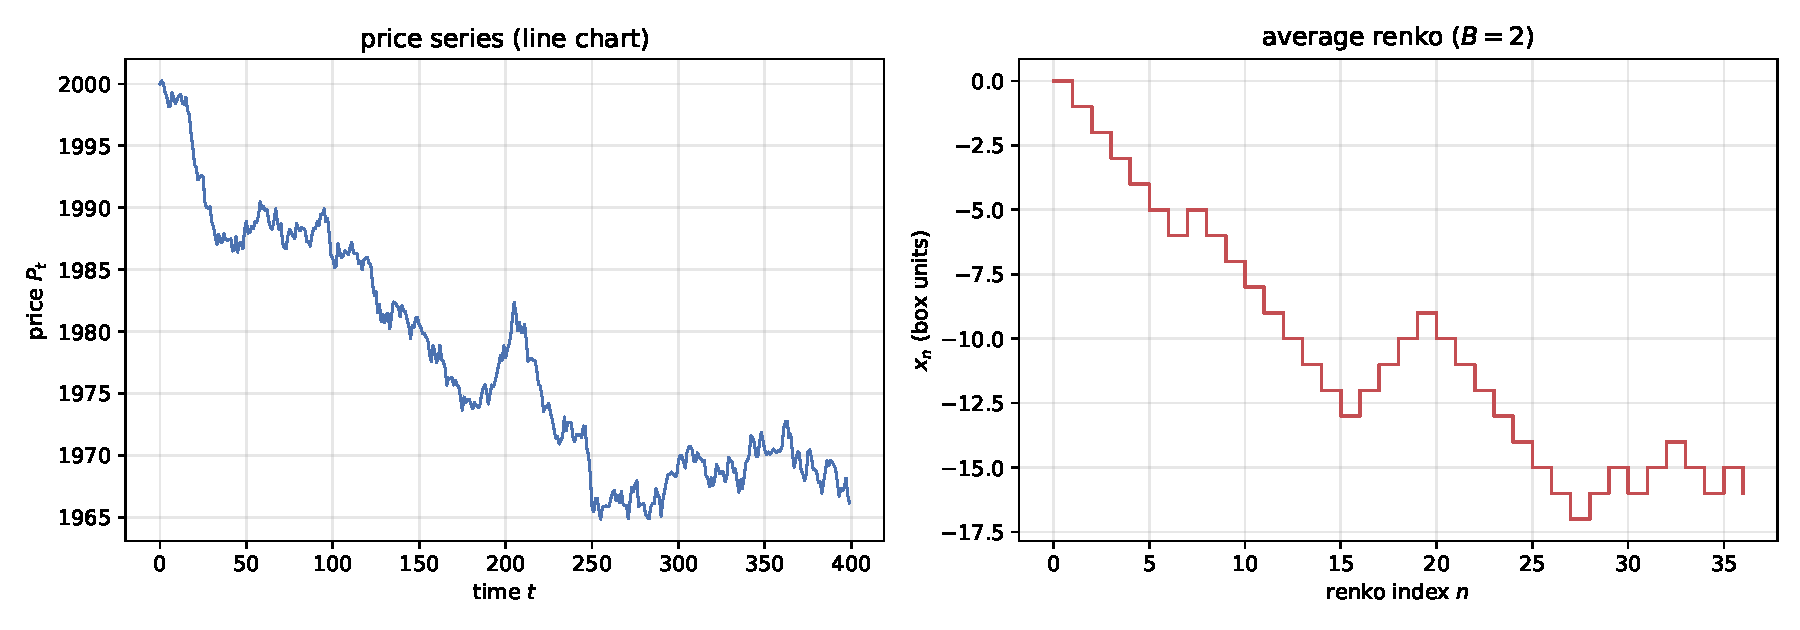
\includegraphics[width=\textwidth]{linechart_renko_compare}
  \caption{価格系列から平均練行足への変換例}
  \label{fig:linechart_renko_compare}
\end{figure}
\newpage
\section{実験結果}

\subsection{実験設定}\label{subsec:exp_setup}

本章では，本研究で構成した相関付きランダムウォークに基づく時系列モデルを
XAUUSD の実価格データに適用し，その予測性能を評価する。
以下ではまず実験の設定を述べ（\ref{subsec:exp_setup}節），
次に第5章で構成したモデルをそのまま，すなわち過去の全期間を参照して
実データに当てはめた結果をベースラインとして示す（\ref{subsec:full_baseline}節）。
この結果は，全期間参照のままでは予測としての妥当性が低いことを示す。
そこで，予測に用いる直近の観測点の個数（\textbf{参照期間}）$W$ を導入して
モデルの当てはめ方を改良し（\ref{subsec:rolling}節），
$W$ を系統的に変えたときの予測誤差と計算時間の変化を
主実験として調べる（\ref{subsec:w_sweep}節以降）。
本実験で調整するパラメータは，この参照期間 $W$ のみである。

用いる原データは XAUUSD の1分足価格系列である。
実験には目的に応じて複数の区間を用いるが，本章の主実験では代表として
2026年6月29日23時22分から同月30日4時38分（UTC，1分足317本）の区間を対象とする。
値幅 $B$ は，離散化後も値動きの特徴（トレンドや持ち合いの形）が失われないよう，
対象区間の変動幅に応じて適宜定める。本区間では $B=3$（ドル）とし，
前章で述べた手順に従って平均練行足を構成して
符号列 $b_1,\ldots,b_N$（$N=156$ 本）と
これを累積した整数時系列 $x_n$（$x_0=0$）を解析の入力とする。
符号列の $+1$（上昇）の比率は $0.474$，
直前と逆符号になった遷移の比率（以下，\textbf{反転率} $\hat{r}$）は $\hat{r}=0.381$，
同符号が連続する本数（連長）の平均は $2.6$ 本（最大 $14$ 本）であり，
これらの統計量は考察（第8章）で参照する。

評価関数 $V_n(p,q,\alpha)$（式\eqref{eq:model_Vn}）の最小化は，
本章を通じて $p,q,\alpha\in\{0,\,0.1,\,0.2,\ldots,1\}$ の格子
（$11^3=1331$ 点）上の全探索によって行い，
最小値との差が $10^{-10}$ 以下の格子点をすべて最小解とみなして
式\eqref{eq:model_prediction_multiple} の平均をとる。
この操作を各時刻について繰り返し，予測列 $x_1^{\ast},\ldots,x_N^{\ast}$ を得る。

\subsubsection*{評価指標}

本研究では予測値 $x_n^{\ast}$ と実測値 $x_n$ を同一図に重ねて描き，
予測が値動きに追従できているかを視覚的に確認することを評価の中心とする。
これは，本実験の関心が誤差の大小そのものよりも，
値動きの継続や転換といった局面ごとの予測の振る舞いにあるためである。
あわせて，補助的な定量指標として，予測値と実測値の平均絶対誤差
\begin{equation}
  \mathrm{MAE}=\frac{1}{N}\sum_{n=1}^{N}\lvert x_n-x_n^{\ast}\rvert
  \label{eq:mae}
\end{equation}
を併記する。
MAE（Mean Absolute Error）は予測値と実測値のずれの平均的な大きさを表す指標であり，
誤差の単位がデータと同じで解釈しやすいことから，
気象予報や需要予測，金融時系列の予測など，
予測モデルの精度評価に広く用いられている。
練行足は毎ステップ必ず $\pm1$ 動くため，
直前の値をそのまま予測する「変化なし」予測の MAE は常に $1$ となる。
したがって $\mathrm{MAE}<1$ は，予測が「変化なし」予測よりも誤差が小さいことの目安となる。

また，予測が次の 1 本の方向（上昇・下降）を当てられたかを測る指標として，
\textbf{方向的中率}
\begin{equation}
  \mathrm{HIT}
  =
  \frac{1}{N-1}
  \sum_{n=2}^{N}
  \mathbf{1}\bigl\{
    \mathrm{sgn}(x_n-x_{n-1})
    =
    \mathrm{sgn}(x_n^{\ast}-x_{n-1})
  \bigr\}
  \label{eq:hit}
\end{equation}
を用いる。ここで $\mathbf{1}\{\cdot\}$ は条件が成り立つとき $1$，
成り立たないとき $0$ をとる指示関数，$\mathrm{sgn}$ は符号関数である。
実測値は毎ステップ必ず $\pm1$ 動くため，方向を無作為に選ぶ予測の HIT は $0.5$ となる。
したがって $\mathrm{HIT}>0.5$ が，方向予測として意味をもつことの目安となる。

さらに，本章では参照期間 $W$ が計算量に与える影響も調べるため，
各 $W$ について予測列 $x_1^{\ast},\ldots,x_N^{\ast}$ の計算に要した実時間を記録する。
計測は Google Colaboratory 上の CPU 実行によるものであり，
同一の足系列・同一の計算環境で $W$ のみを変えて行い，
系列全体の総計算時間と，1 ステップ（1 回の予測）当たりの平均時間を報告する。
計算時間は予測の質を表す指標ではなく，
モデルを運用する際の実用上のコストとして参照する。

\subsection{全期間参照によるベースライン評価}\label{subsec:full_baseline}

まず，参照期間を区切らず，各時刻 $n$ で過去の全期間 $D_n$ を用いて当てはめる場合，
すなわち第5章で構成したモデルそのもの（式\eqref{eq:model_prediction}）を，
\ref{subsec:exp_setup}節の実データに適用した。結果は
\[
  \mathrm{MAE}=5.94,
  \qquad
  \mathrm{HIT}=0.43
\]
であった。
MAE は「変化なし」予測の基準値 $1$ の約 $6$ 倍であり，
HIT は方向を無作為に選ぶ予測の基準値 $0.5$ をも下回る。
すなわち，全期間参照のモデルは誤差・方向のいずれの観点でも
自明な基準予測に劣り，このままでは金価格の値動きの予測として妥当性が低い。

% ★図の差し替え待ち：実測 x_n と全期間参照の予測 x_n* の重ね図（実データ）。
% 生成方法: run_multi_w_overlay(path, B=3, windows=["full"]) の図，または
% run_batch_collection の batch_0000.png と同等のもの。PNG を docs/thesis/
% に full_baseline_overlay.png として置き，以下のコメントを外す。
% 図が入ったら，直前の段落に「予測と実測の乖離のようす（図参照）」への言及を加える。
\begin{figure}[H]\centering
 \includegraphics[width=\textwidth]{batch_0000}
 \caption{実測 $x_n$ と全期間参照による予測 $x_n^{\ast}$ の重ね描き}
 \label{fig:full_baseline_overlay}
\end{figure}

この失敗の原因は，次のように考えられる。
全期間参照による当てはめは，系列全体が単一のパラメータ $(p,q,\alpha)$ から
定常に生成されているという仮定に相当する。
しかし実際の値動きは，上昇・下降・持ち合いといった局面が切り替わる
非定常な系列であり，既に終わった局面の観測が推定に混入し続けるため，
現在の局面に対する予測が系統的にずれていく
（機構の詳細は第8章で考察する）。

そこで以下では，当てはめに用いる観測を\textbf{直近 $W$ 点に限る}
という改良を加え，この参照期間 $W$ が予測性能をどう変えるかを調べる。

\subsection{参照期間の導入}\label{subsec:rolling}

参照期間 $W$ とは，予測に用いる直近の観測点の個数である
（足の本数では $W-1$ 本に相当する）。
時刻 $n$（$n\geq W-1$）における予測は，次の手順で行う。
まず，直近 $W$ 点の部分系列を取り出し，先頭の値を引いて再基準化した系列
\begin{equation}
  y_j=x_{n-W+1+j}-x_{n-W+1}
  \qquad (j=0,1,\ldots,W-1)
  \label{eq:rolling_rezero}
\end{equation}
を作る。$y_0=0$ であり，各増分は $\pm1$ なので，
$y_0,\ldots,y_{W-1}$ は第5章の観測データの規約（式\eqref{eq:model_x0}〜\eqref{eq:model_bn_pm}）を満たす。
次に，この系列に対して評価関数 $V_{W-1}(p,q,\alpha)$（式\eqref{eq:model_Vn}）を最小化し，
推定パラメータ $(p^\ast,q^\ast,\alpha^\ast)$ を得る。
そして，次時刻の予測値を，窓の先頭を基準とした $W$ ステップ後の期待値
\begin{equation}
  x_{n+1}^{\ast}
  =
  x_{n-W+1}
  +
  E(\tilde{S}_{W}\mid p^\ast,q^\ast,\alpha^\ast)
  \label{eq:rolling_prediction}
\end{equation}
と定める。最小解が複数ある場合・$V$ が定数の場合の扱いは，
式\eqref{eq:model_prediction_multiple}・式\eqref{eq:model_prediction_const} と同様である。
序盤の $n<W-1$ では，その時点で利用できる全履歴 $D_n$ を用いる。
また，参照期間を区切らず $D_n$ 全体を用いる場合，
すなわち前節のベースライン（第5章のモデルそのもの，基準は $x_0=0$）を
\textbf{全期間}とよび，以降では $W$ を有限にとった場合との比較対象とする。

\subsection{参照期間 $W$ に対する感度分析}\label{subsec:w_sweep}

参照期間 $W$ は本実験で唯一の調整パラメータであり，
予測誤差と計算量の双方を左右する。
そこで本節では，$W$ を最小の $W=2$（直近の足 1 本のみを参照）から
全期間まで系統的に変え，MAE と計算時間がどのように変化するかを調べる。
具体的には
\[
  W\in\{2,\,3,\,5,\,10,\,20,\,30,\,60\}\ \text{および全期間}
\]
の 8 通りについて，同一の足系列に対して予測列を計算した。
$W$ の候補は，取り得る最小値である $W=2$ から，
足数十本分の長い履歴に相当する $W=60$ までを，
おおむね倍々の間隔で幅広く覆うように選んだものであり，
個々の値そのものに特別な意味はない。
結果を表\,\ref{tab:w_sweep} および図\,\ref{fig:w_sweep} に示す。

結果はほぼ単調であった。
すなわち，MAE は最小の $W=2$ で最も小さく（$0.847$），
$W$ とともに概ね単調に増加して全期間で最大（$5.94$，
\ref{subsec:full_baseline}節のベースラインに一致）となった
（例外は $W=20$ から $W=30$ にかけての小さな逆転のみである）。
計算時間は $W$ に対して単調に増加した。
したがって，\textbf{小さい参照期間が誤差・計算時間の両面で優位であり，
精度と計算量のあいだのトレードオフは観測されなかった}。
MAE が「変化なし」予測の基準値 $1$ を下回るのは $W=2$（$0.847$）と
$W=3$（$0.979$）のみであった。

計算時間が $W$ とともに増加することは，モデルの構造からも説明できる。
1 回の予測では，格子上の $1331$ 点それぞれについて
確率分布の時間発展（式\eqref{eq:crw_evolution}）を $W-1$ ステップ計算するため，
1 ステップ当たりの計算量は $W$ の増加に伴いおよそ 2 乗のオーダーで増える
（時刻 $t$ の分布の台が $2t+1$ 点に広がるため）。
全期間では参照長が $n$ とともに増えるので，系列全体では更に大きくなる。
分布の計算を時刻間で使い回すなどの実装上の工夫により定数倍の改善は可能だが，
計算量が $W$ について単調に増えること自体は変わらない。

\begin{table}[H]\centering
  \caption{参照期間 $W$ ごとの予測誤差と計算時間}
  \label{tab:w_sweep}
  \begin{tabular}{l|cccccccc}\hline
    指標 & $W=2$ & $W=3$ & $W=5$ & $W=10$ & $W=20$ & $W=30$ & $W=60$ & 全期間 \\\hline
    MAE & 0.847 & 0.979 & 1.202 & 1.455 & 2.072 & 1.882 & 3.009 & 5.941 \\
    総計算時間 [s] & 7.7 & 11.5 & 18.1 & 34.4 & 62.6 & 91.7 & 174.5 & 310.9 \\
    1ステップ当たり [ms] & 49 & 74 & 116 & 220 & 401 & 588 & 1118 & 1993 \\\hline
  \end{tabular}
\end{table}

\begin{figure}[H]\centering
  \includegraphics[width=\textwidth]{w_sweep_summary}
  \caption{参照期間 $W$ に対する MAE（左）と 1 ステップ当たり計算時間（右）。
  左図の破線は「変化なし」予測の基準 $\mathrm{MAE}=1$ を表す。}
  \label{fig:w_sweep}
\end{figure}

\subsection{実測値と予測値の重ね描き}\label{subsec:w_overlay}

前節の表は誤差を集計した値であり，
予測がどのような場面で当たり，どのような場面で外れているかまでは分からない。
そこで評価の中心である視認比較として，
参照期間の小・中・大を代表する $W=2,\,10,\,60$ の 3 通りについて，
予測値 $x_n^{\ast}$ を実測値 $x_n$ と同一図に重ねた結果を
図\,\ref{fig:w_overlay} に示す
\footnote{序盤の $n<W-1$ では全履歴を参照するため（\ref{subsec:rolling}節の予測手順），
各系列の違いは $n\geq W-1$ 以降に現れる。}。

% ★仮置きの図に基づく記述：実データの図に差し替えたら本段落も図に合わせて書き直す。
$W=2$ の予測は，直前の値動きをなぞる形で実測値のごく近くを推移し，
値動きの継続にも転換にも数本以内で追従した。
$W=10$ もこれに近い軌跡を描いた。
一方 $W=60$ の予測は，レンジから上昇へ移る局面ではレンジ局面の情報を引きずって
実測値の下に取り残され，
天井をすぎて下降へ転じる局面では逆に上昇の傾きを引きずって実測値の上方へ乖離した。
このような局面の変わり目ごとに生じる乖離の累積が，
前節で見た「$W$ が大きいほど MAE が大きい」という傾向に対応している。

% ★仮置き（合成データによる暫定図）：実データ入手後に
% colab/oyosuri_experiment.py の run_multi_w_overlay(..., windows=[2,10,60]) で差し替える。
% 実データで点数が多く見にくい場合は代表的な区間の抜粋に差し替えてもよい。
\begin{figure}[H]\centering
  \includegraphics[width=\textwidth]{w_overlay}
  \caption{実測 $x_n$ と $W=2,10,60$ の予測の重ね描き}
  \label{fig:w_overlay}
\end{figure}

\subsection{局面別の分析}\label{subsec:patterns}

前節までで，参照期間 $W$ が小さいほど誤差が小さいという傾向を確認した。
本節では，この $W$ による差が値動きのどのような局面で生じるのかを調べる。
本モデルは値動きの上昇方向と下降方向を対称に扱うため，
下降局面における予測は対応する上昇局面の予測を上下反転したものとなる。
そこで上昇局面のライフサイクルに対応する次の4パターンを代表例として取り上げる。

実データから局面を切り出すと，区間ごとに足の本数が揃わず比較が難しい。
そこで本節では，実データの練行足の見た目に合わせた簡易な確率モデルを用いて，
長さを $N=150$ 本に揃えた\textbf{合成データ}の符号列を各パターンについて生成し，
これに対する予測の振る舞いを調べる。
生成規則は次のとおりである。
トレンド局面では，直前と同じ方向を確率 $0.70$ で継続し，
逆方向にいる場合は確率 $0.58$ でトレンド方向へ引き戻される
（1 本当たり平均約 $+0.3$ のドリフトをもつ）。
レンジ局面では，局面開始時の水準 $x_{\mathrm{a}}$ への平均回帰
$P(\text{上昇})=0.5-0.09\,(x_n-x_{\mathrm{a}})$
（ただし $0.12$〜$0.88$ に制限）に従い，おおよそ $\pm 5$ 本の帯にとどまる。
2 つの局面からなるパターンは，前半と後半で局面を切り替える。

各パターンについて $W=2,\,10,\,60$ の予測を実測値と同一図に重ねて示し，
各区間の MAE を表\,\ref{tab:pattern_summary} にまとめる。


\subsubsection*{上昇継続}
図\,\ref{fig:pat_uptrend} に示す。
上昇が継続する局面でも，値動きは一直線ではなく押し（一時的な戻り）を挟む。
小さい $W$ の予測は上昇にも押しにも数本の遅れで追従した（$W=2$ で MAE $0.996$）。
一方，$W$ の大きい予測は押しの局面でも直前までの上昇の傾きを引きずって上振れを続け，
$W=60$ では MAE が $4.247$ まで悪化した。
上昇という大きな方向が同じでも，経路が曲がるたびに大きい $W$ の乖離が蓄積することがわかる。
\begin{figure}[H]\centering
  \includegraphics[width=\textwidth]{pat_uptrend_w}
  \caption{上昇継続：実測 $x_n$ と $W=2,10,60$ の予測（合成データ）}
  \label{fig:pat_uptrend}
\end{figure}

\subsubsection*{レンジ→上昇}
図\,\ref{fig:pat_range2up} に示す。
レンジ局面では方向の持続が乏しいため，順張り的に振る舞う小さい $W$ の優位は小さく，
$W=2$（MAE $1.082$）と $W=10$（MAE $1.124$）はほぼ同等で，
いずれも基準値 $1$ をわずかに上回った。
一方，終盤の上昇への転換では $W=60$ の予測が立ち上がりに乗り遅れて
実測値の下に取り残され，区間全体では MAE $2.442$ と差が開いた。
\begin{figure}[H]\centering
  \includegraphics[width=\textwidth]{pat_range2up_w}
  \caption{レンジ→上昇：実測 $x_n$ と $W=2,10,60$ の予測（合成データ）}
  \label{fig:pat_range2up}
\end{figure}

\subsubsection*{上昇→レンジ}
図\,\ref{fig:pat_up2range} に示す。
上昇からレンジへ移ると，$W$ の大きい予測は上昇局面の傾きを引きずり，
レンジ入り後もしばらく実測値の上方へ乖離を続けた（$W=60$ で MAE $2.963$）。
$W=2$ は数本で持ち合いに対応し，MAE は $0.996$ と基準値 $1$ をわずかに下回った。
\begin{figure}[H]\centering
  \includegraphics[width=\textwidth]{pat_up2range_w}
  \caption{上昇→レンジ：実測 $x_n$ と $W=2,10,60$ の予測（合成データ）}
  \label{fig:pat_up2range}
\end{figure}

\subsubsection*{上昇→下降}
図\,\ref{fig:pat_up2down} に示す。
上昇から下降へ転じる局面では $W$ による差が4パターン中で最も大きい。
$W=60$ の予測は天井を過ぎたあとも長く上昇方向の予測を出し続け，
実測値から大きく乖離した（MAE $4.876$）。
$W=2$ は反転から数本で下降方向へ切り替わり，
MAE は $0.892$ と4パターン中で最小であった。
\begin{figure}[H]\centering
  \includegraphics[width=\textwidth]{pat_up2down_w}
  \caption{上昇→下降：実測 $x_n$ と $W=2,10,60$ の予測（合成データ）}
  \label{fig:pat_up2down}
\end{figure}

各パターン・各参照期間の MAE と HIT を表\,\ref{tab:pattern_summary} にまとめる。
MAE はいずれのパターンでも $W=2<W=10<W=60$ の順であり，
$W$ が小さいほど誤差が小さい。
一方，HIT は $W=2$ でも $0.44$〜$0.58$ とおおむね $1/2$ 前後にとどまり，
MAE ほど明確な差は現れなかった。

\begin{table}[H]\centering
  \caption{各パターン・各参照期間の MAE と HIT（合成データ，$N=150$）}
  \label{tab:pattern_summary}
  \begin{tabular}{l|ccc|ccc}\hline
    & \multicolumn{3}{c|}{MAE} & \multicolumn{3}{c}{HIT} \\
    パターン & $W=2$ & $W=10$ & $W=60$ & $W=2$ & $W=10$ & $W=60$ \\\hline
    上昇継続     & 0.996 & 1.407 & 4.247 & 0.50 & 0.44 & 0.37 \\
    レンジ→上昇 & 1.082 & 1.124 & 2.442 & 0.44 & 0.52 & 0.50 \\
    上昇→レンジ & 0.996 & 1.368 & 2.963 & 0.50 & 0.44 & 0.47 \\
    上昇→下降   & 0.892 & 1.485 & 4.876 & 0.58 & 0.46 & 0.40 \\\hline
  \end{tabular}
\end{table}

\subsubsection*{乱数系列に対する頑健性}
以上の結果が特定の乱数系列に依存しないことを確認するため，
同一のパターン設定で乱数系列のみを変えた第2のインスタンスを生成し，
同じ比較を行った。
MAE の順序 $W=2<W=10<W=60$ は，
2インスタンス $\times$ 4パターンの全8ケースで成立し，
第2インスタンスでは $W=2$ の MAE は全パターンで $1$ を下回った。
すなわち，小さい $W$ の優位は乱数系列によらず MAE の順序として頑健に現れる。
一方，HIT の細部は乱数系列に依存する。
第1インスタンス（表\,\ref{tab:pattern_summary}）では
$W=2$ の HIT は $0.44$〜$0.58$ と $1/2$ 前後にとどまったのに対し，
方向の持続がより強く現れた第2インスタンスでは $0.53$〜$0.60$ であった。
これは，$W=2$ の予測が直近の方向をほぼそのまま引き継ぐため，
その的中率が系列自体の方向の持続の強さを反映して変わることによる。
したがって，HIT の値そのものは系列の性質に応じて変動する量であり，
モデル固有の性能とは切り離して解釈する必要がある。
\newpage
\section{考察}
前章の実験で得られた主な結果は，次の3点に整理できる。
第一に，全期間参照によるベースラインは
$\mathrm{MAE}=5.94$，$\mathrm{HIT}=0.43$ であり，
誤差・方向のいずれの観点でも自明な基準予測を下回った。
第二に，参照期間 $W$ が小さいほど予測誤差も計算時間も小さく，
精度と計算量のトレードオフは観測されなかった。
この MAE の順序は，局面別の合成データでも，乱数系列を変えても
保たれる頑健な傾向であった。
第三に，MAE とは対照的に，HIT は $W$ によらずおおむね $1/2$ 前後にとどまり，
$W$ による明確な優劣は現れなかった。
本章では，これらの結果が本モデルのどのような構造から生じるのかを検討し，
そのうえで本モデルの妥当性と限界を整理する。

\subsection{参照期間依存性が生じる機構}

まず，誤差が $W$ とともに増える理由を予測値の構成から考える。
参照期間 $W$ の予測値（式\eqref{eq:rolling_prediction}）は，
窓の先頭 $x_{n-W+1}$ を基準とした $W$ ステップ後の期待値であり，
現在位置 $x_n$ や直前の方向を\textbf{条件としていない}。
すなわち，予測は「窓の先頭から眺めた $W$ 歩先の平均的な到達点」であり，
現在位置からの 1 歩を直接推定しているわけではない。

評価関数の構造もこの点と関わる。
式\eqref{eq:model_Vn} の内側の和は，期待値のまわりの分解
\begin{equation}
  \sum_{x=-t}^{t}(x-x_t)^2\,\mu_t(x;p,q,\alpha)
  =
  \mathrm{Var}(\tilde{S}_t)
  +
  \bigl(E(\tilde{S}_t)-x_t\bigr)^2
  \label{eq:Vn_decomp}
\end{equation}
と書き直せる。
第 1 項（分散項）は観測値によらず時刻 $t$ とともに増えるため，
最小化は分散の小さい，すなわちできるだけ確定的なパラメータを選ぶ方向に働く。
第 2 項（平均項）は遅い時刻ほど重みが大きく
（期待値経路の傾きのずれ $\delta$ は $(\delta t)^2$ で効く），
当てはめは窓の終端寄りの観測に期待値経路を沿わせる。
結果として，参照期間 $W$ の予測は，
窓内の $W$ 点を 1 本の傾きで近似してその先へ延長する，
直線的な外挿に近い振る舞いになる。

このとき予測誤差は，窓内の経路が 1 本の直線からどれだけ外れているかに支配され，
それは $W$ とともに増える。
第一に，方向の定まらない区間では，位置の揺らぎの幅は
時間幅の平方根のオーダーで増える（第4章の定理\,\ref{thm:clt_corr} のスケーリング）。
第二に，窓の途中に局面の転換が入ると，転換前の情報がおよそ $W$ 本ぶん参照され続けるため，
追従の遅れが $W$ に比例して長引く。
\ref{subsec:patterns}節の局面別分析は，この第二の機構と対応している。
すなわち，転換が最も急な上昇→下降では $W$ 間の差が4パターン中で最大となり
（$W=2$ の MAE $0.892$ に対し $W=60$ は $4.876$，表\,\ref{tab:pattern_summary}），
転換を含まないレンジ局面では $W=2$ と $W=10$ の差はほとんど生じなかった。
全期間参照では基準が常に $x_0$ であり，
局面をまたいだずれが解消されずに蓄積するため，誤差は最も大きくなる。
このように，「$W$ が小さいほど誤差が小さい」という実験結果は，
偶然ではなく，無条件期待値に基づく予測という本モデルの構成そのものに由来すると考えられる。

\subsection{練行足系列の記憶の長さ}

データの側からも同じ結論が支持される。
本モデルは増分について 1 次マルコフ的であり，
次の方向に影響するのは直前の方向のみである。
一方，実験に用いた符号列では反転率が $\hat{r}=0.381$，
同符号の連長は平均 $2.6$ 本であった。
すなわち同じ方向が続く長さは平均数本であり，
数本より前の足は現在の方向とほとんど相関をもたない。
したがって参照期間を延ばしても新しい情報はほとんど加わらず，
むしろ既に終わった局面の足が推定に混入して，
現在の局面に対するパラメータ推定を薄める
（長い参照期間は，系列が定常であるという仮定を強める操作だが，
実際の値動きは局面が切り替わる非定常な系列である）。
この意味で，短い参照期間が有利という結果は，
練行足系列の記憶の短さとも整合している。

\subsection{小さい参照期間の極限と順張り予測}

参照期間を最小の $W=2$ までつめると，本モデルの振る舞いは明示的に書ける。
このとき再基準化した窓は $(y_0,y_1)=(0,\,b_n)$ であり，
$\tilde{S}_1^2=1$，$y_1^2=1$ に注意すると評価関数は
\begin{equation}
  V_1(p,q,\alpha)
  =
  E\bigl[(\tilde{S}_1-y_1)^2\bigr]
  =
  2-2\,b_n\,E(\tilde{S}_1)
  \label{eq:V1_closed}
\end{equation}
となる。
これを最小にするのは $E(\tilde{S}_1)=b_n$，
すなわち\textbf{確率 $1$ で直前と同じ方向へ進む}パラメータの組すべてであり，
予測値はそれらの期待値の平均（式\eqref{eq:model_prediction_multiple}）として
\[
  x_{n+1}^{\ast}\approx x_n+\gamma\,b_n
  \qquad (0<\gamma<1)
\]
の形になる（本実験の格子では $\gamma=0.645$）。
これは「直前と同じ方向へ動く」と読む\textbf{順張り予測}を，
複数解の平均によって係数 $\gamma$ に縮小したものにほかならない。

この形から，$W=2$ における本モデルの MAE は閉形式で書ける。
継続（確率 $1-\hat{r}$）では誤差 $1-\gamma$，
反転（確率 $\hat{r}$）では誤差 $1+\gamma$ を出すから，
\begin{equation}
  \mathrm{MAE}
  =
  (1-\hat{r})(1-\gamma)+\hat{r}(1+\gamma)
  =
  (1-\gamma)+2\gamma\hat{r}
  \label{eq:mae_w2}
\end{equation}
である。実験系列の反転率 $\hat{r}=0.381$ を代入すると
$(1-0.645)+2\times0.645\times0.381=0.846$ となり，
実測の $\mathrm{MAE}=0.847$（表\,\ref{tab:w_sweep}，$W=2$）とほぼ一致する
（わずかな差は，履歴が 1 点しかない序盤のステップが
式\eqref{eq:model_prediction_const} の「変化なし」予測となることによる）。
すなわち，誤差が最小となる設定における本モデルの振る舞いは，
縮小した順張り予測として定量的に説明し尽くされる。

一方，縮小しない順張り予測そのもの（$x_{n+1}^{\ast}=x_n+b_n$）の MAE は，
継続で $0$，反転で $2$ の誤差を出すから $2\hat{r}$ であり，
実験系列では $2\hat{r}=0.761$ となる。
これは本モデルの最良値 $0.847$ よりも小さい。
実際，式\eqref{eq:mae_w2}より，$\hat{r}<1/2$（持続性のある系列）では
$(1-\gamma)+2\gamma\hat{r}>2\hat{r}$ が任意の $0<\gamma<1$ について成り立ち，
予測の縮小はかえって誤差を増やす。
すなわち，本モデルは誤差最小の設定でも，
「変化なし」予測（$\mathrm{MAE}=1$）には勝つものの，
単純な順張り予測を MAE の意味で上回ることはできなかった。
一方で本モデルは，予測を期待値という連続値で返すため確信の強さが値の大きさに現れ，
また推定パラメータ $p,q$ によって持続性・反転傾向の強さを局面ごとに定量化できる。
この点で，単に方向を当てるだけの順張り予測より多くの情報を与える枠組みだといえる。

\subsection{MAE と HIT の乖離}\label{subsec:mae_hit_gap}

前章の結果では，MAE で見た小さい $W$ の優位は，
実データの感度分析（表\,\ref{tab:w_sweep}）でも，
局面別の合成データ（表\,\ref{tab:pattern_summary}）でも，
乱数系列を変えた第2インスタンスでも一貫して現れた。
一方，HIT は $W=2$ でも $0.44$〜$0.58$ と $1/2$ 前後にとどまり，
その値は乱数系列によって変わった。
この MAE と HIT の乖離は，前節の $W=2$ の閉形式から説明できる。

$W=2$ の予測は $x_{n+1}^{\ast}\approx x_n+\gamma\,b_n$ であり，
予測の\textbf{方向}は直前の方向 $b_n$ そのものである。
したがって $W=2$ の HIT は，系列が直前と同じ方向へ動き続けた割合，
すなわち継続率 $1-\hat{r}$ をほぼそのまま映す。
合成データの第2インスタンスで HIT が $0.53$〜$0.60$ へ上がったのは，
その系列で方向の持続がより強く現れたためであって，
モデルが方向を見抜く能力を獲得したためではない。
この意味で，HIT はモデルの能力というより
対象系列の持続性の測定値として振る舞う。

したがって，本モデルの優位が現れるのは方向の的中ではなく，
\textbf{予測が実測から大きく乖離しないこと}，
すなわち MAE の側である。
小さい $W$ は，大きい $W$ が局面転換のたびに起こす
外挿の乖離の蓄積を抑えることで誤差を小さくしており，
これが乱数系列や局面によらず MAE の順序が頑健に保たれた理由である。
全期間参照の HIT が $0.43$ と $1/2$ を下回ったことも，
終わった局面の方向を引きずって方向判定が系統的に遅れるという
同じ機構の現れとして整合的に説明できる。

なお，前章で見たとおり精度と計算量のあいだにトレードオフはなく，
小さい $W$ は誤差・計算時間の両面で優位である。
したがって，本モデルを運用する際に小さい $W$ を選ぶことは，
実用上も合理的な選択である。

\subsection{本モデルの妥当性と限界}

以上を踏まえ，序論で掲げた問い（本モデルが金価格の値動きを記述するうえでの
妥当性と限界）に対する本研究の答えを整理する。

\textbf{妥当性}について。
小さい参照期間では MAE が「変化なし」予測の基準値 $1$ を下回り，
重ね描きでも予測が値動きの継続・転換に短い遅れで追従することが確認された。
すなわち，練行足化によって値動きを $\pm1$ の系列に離散化し，
直前の方向への依存（持続性）を相関付きランダムウォークで表すという本研究の枠組みは，
金価格の値動きがもつ短期の方向の持続を捉える目的に対して一定の妥当性をもつ。

\textbf{限界}について。
第一に，予測が現在位置を条件としない期待値で構成されるため，
参照期間を延ばすほど精度が下がり，長い履歴を活かす仕組みをモデル自身がもたない。
有効に使える記憶は実質的に直近数本に限られる。
第二に，その帰結として転換局面に弱く，
誤差最小の設定での振る舞いは縮小した順張り予測に帰着し，
本データでは単純な順張り予測（$\mathrm{MAE}=2\hat{r}=0.761$）を
上回ることができなかった。
また，方向的中率 HIT の観点では，どの参照期間でも $1/2$ を明確に超える
的中率は得られず，方向予測としての優位は示せなかった
（\ref{subsec:mae_hit_gap}節）。
第三に，本研究の結果には次の留保が付く。
対象は単一資産・単一期間であり，値幅 $B$ も 1 通りに固定している
（練行足の構造，したがって結果は $B$ の取り方に依存し得る）。
参照期間 $W$ の比較は同一系列上の誤差で行っており，
運用上は $W$ を事前に決める必要がある。
パラメータ探索の格子は分解能 $0.1$ であり，
計算時間の絶対値は実装に依存する（ただし $W$ に関する単調性は実装によらない）。
また局面別の分析は合成データによる確認であり，
実データの個々の局面で同じ振る舞いとなるかは別途確認を要する。

\section{今後の課題}

本研究の結果から，今後の課題として次の点が挙げられる。

\begin{itemize}
  \item \textbf{現在位置・直前の方向を条件とする予測への拡張}：
        本モデルの誤差の主因は，予測が無条件期待値で構成される点にあった。
        時刻 $n$ の位置と向きを条件とした条件付き期待値
        $E(\tilde{S}_{n+1}\mid \tilde{S}_n=x_n,\ \text{直前の向き})$
        を予測値に用いる定式化に改めれば，
        参照期間を延ばしたときの劣化を抑えられる可能性がある。
  \item \textbf{参照期間の適応的な選択}：
        本研究では $W$ を固定したが，局面の転換を検出して
        $W$ を切り替える適応的な方法が考えられる。
  \item \textbf{頑健性の確認}：
        値幅 $B$・対象資産・対象期間を変えた追試，
        およびパラメータ（$W$ など）の選択に用いる区間と
        評価に用いる区間を分けた検証により，
        本研究で得られた傾向の一般性を確かめる必要がある。
  \item \textbf{局面別分析の実データへの拡張}：
        本研究の局面別分析は合成データによった。
        実データから局面を客観的に切り出す基準を定式化し，
        実データ上でも同じ振る舞いを確認することが望ましい。
  \item \textbf{計算の効率化}：
        確率分布の時間発展はパラメータごとに毎時刻計算し直しており，
        分布の再利用などの実装上の工夫で計算時間を大きく削減できる。
  \item \textbf{量子ウォークに基づく時系列モデルとの比較}：
        本モデルの構成のもととなった Konno~\cite{ref3} の量子ウォーク版と
        同一データ・同一手順で比較し，
        相関付きランダムウォークを用いることの利点と欠点を明らかにする。
\end{itemize}



\newpage
\begin{thebibliography}{9}

\bibitem{ref3}
  N.~Konno,
  A new time-series model based on quantum walk,
  Quantum Studies: Mathematics and Foundations, \textbf{6}, 61--72 (2019).
  % DOI: 10.1007/s40509-018-0162-1

\bibitem{ref1}
  % TODO: 書誌情報を記入（第3章の大数の法則・中心極限定理，および
  % 第4章の命題（対称性）の出典として参照した教科書）
  著者名，『書名』，出版社（出版年）．

\bibitem{ref2}
  % TODO: 書誌情報を記入（第4章の相関付きランダムウォークの弱収束極限定理で参照した文献）
  著者名，論文題目，誌名，\textbf{巻}，頁（出版年）．

\end{thebibliography}
\newpage
\section{付録}
\end{document}
